% This file was created with tikzplotlib v0.10.1.
\definecolor{mycolor1}{rgb}{0.00000,0.44700,0.74100}%
\definecolor{mycolor2}{rgb}{0.85000,0.32500,0.09800}%
\definecolor{mycolor3}{rgb}{0.92900,0.69400,0.12500}%
\definecolor{mycolor4}{rgb}{0.49400,0.18400,0.55600}%

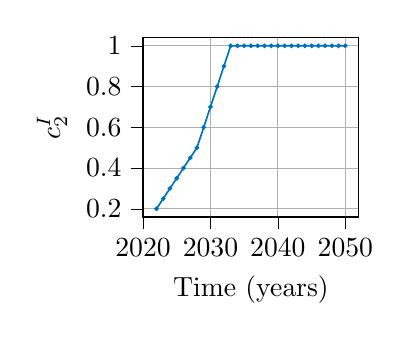
\begin{tikzpicture}

\definecolor{darkgray176}{RGB}{176,176,176}
\definecolor{steelblue31119180}{RGB}{31,119,180}

\begin{axis}[
scale=0.4,
/pgf/number format/1000 sep={},
tick align=outside,
tick pos=left,
x grid style={darkgray176},
xlabel={Time (years)},
xmajorgrids,
xmin=2020, xmax=2052,
xtick style={color=black},
y grid style={darkgray176},
ylabel={$c_2^I$},
ymajorgrids,
ymin=0.16, ymax=1.04,
ytick style={color=black}
]
\addplot [semithick, mycolor1, mark=*, mark size=.5, mark options={solid}]
table {%
2022 0.2
2023 0.25
2024 0.3
2025 0.35
2026 0.4
2027 0.45
2028 0.5
2029 0.6
2030 0.7
2031 0.8
2032 0.9
2033 1
2034 1
2035 1
2036 1
2037 1
2038 1
2039 1
2040 1
2041 1
2042 1
2043 1
2044 1
2045 1
2046 1
2047 1
2048 1
2049 1
2050 1
};
\end{axis}

\end{tikzpicture}
